\section{System architecture}
\label{sec:architecture}
\thispagestyle{fancy}
The system is designed around three major data structures, or indices. These are the occurrence index which store inverted lists with positions. The content index stores the content of the documents, and is used for snippets and clustering. The last index is the statistics index which is used to store document statistics which may be used to calculate relevance. 

All these indices are wrapped by one class \texttt{SearchEngineMaster}. The external interface for the system uses this master class to feed documents and to execute queries.  

\subsection{Statistics index structure}\label{sub:statistics_index_structure}
The statistics index is a mapping from document id to a statistics object containing information such as most frequent term, document vector $tf*idf$ length and number of unique terms.

\subsection{Content index structure}\label{sub:content_index_structure}
The content index stores the content of the documents indexed, these documents are stored as lists of tokens. These are the raw tokens of the documents nothing is added or removed. By concatenating any consecutive subsequence of these tokens a section of the original document will be produced. This property are used when extracting snippets.  

\subsection{Occurrence index structure}\label{sub:occurrence_index_structure}
The occurrence index consists of two parts, the dictionary and the inverted file. The dictionary contains the terms of documents, and a pointer into the inverted file. The inverted file contains the inverted lists for each term in alphabetical order. The inverted list of a term contains the documents occurrences that contain the term sorted on increasing document id. Each document occurrence contains a list the positions within the document where the term occurred. The index structure is shown in Figure~\ref{fig:occ_index_struct}.

\begin{figure}[h!!tb]
	\centering
	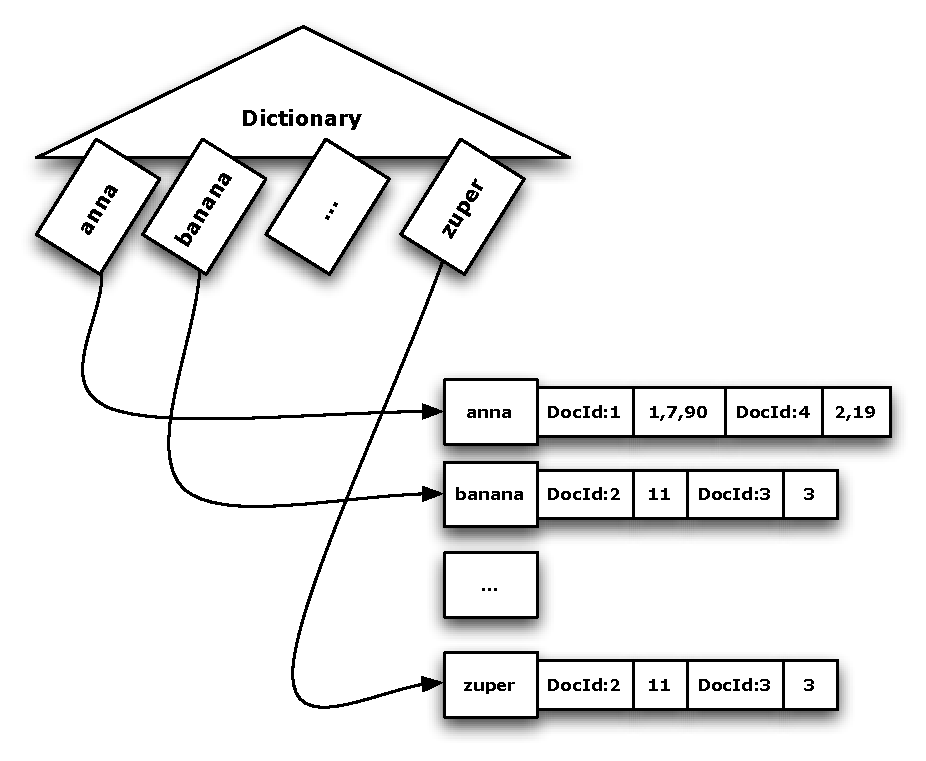
\includegraphics[width=0.8\textwidth]{include/index.pdf}
	\caption[Occurrence index structure]{Occurrence index structure.}\label{fig:occ_index_struct}
\end{figure}

\subsection{Index building}\label{sub:index_building}
When building indices, all documents fed to the system are given a unique document id from a global counter.

The occurrence index is built in two phases, in the first phase documents are converted to inverted lists and combined into one inverted list representing one index update. 

When the index is flushed, the index update that were built in the first phase is merged with the existing inverted index. Since the inverted lists are sorted on term, document and position merging the lists is a trivial task. 

During this merge, the statistics for each document is calculated and stored in the statistics index. 

When the merge is completed the dictionary is updated so that the pointers in the dictionary points into the newly created inverted file. 

\section{Feeding pipeline}\label{sec:feeding_pipeline}
The feeding pipeline of our solution is modeled around two main concepts. A document structure which is a object containing various objects with various keys (fields), it's basically a map. A processor is a processing unit in our feeding pipeline which transforms a field in a document structure, and places the result in another. An example of a feeding processor is shown in Figure~\ref{fig:feeding_processor}.

\begin{figure}[htb]
	\centering
	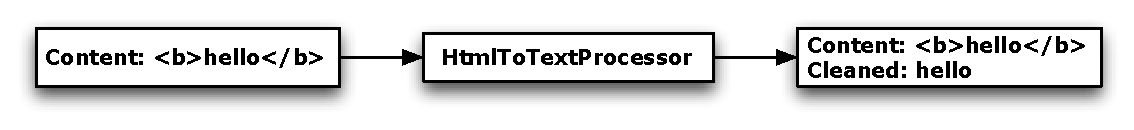
\includegraphics[width=0.9\textwidth]{include/processor.pdf}
	\caption[Feeding pipeline example]{Feeding pipeline example, a html to text processor strips away html from the input field ``content'', and puts the result into the ``cleaned'' field.}\label{fig:feeding_processor}
\end{figure}

\subsection{Implemented feeding processors}\label{sub:implemented_feeding_processors}
To be able to solve our task we have implemented multiple feeding processors. These are:

\begin{itemize}
	\item \textbf{HtmlToText:} strips away HTML tags.
	\item \textbf{Tokenizer:} brakes the documents into tokens. These tokens are the raw tokens of the documents, that is, no characters are removed from the text, the text is only split into pieces.
	\item \textbf{PunctuationRemover:} removes punctuations and whitespaces from tokens. 
	\item \textbf{Stemmer:} reduces tokens to their stems. 
	\item \textbf{Termizer:} creates inverted documents, collecting position lists for each term in the document.
\end{itemize}